\section{Charge Carriers and Doping}

\subsection{Introduction}
We start learning about resistors, capacitors, and inductors from earlier courses such as EECS 16A and 16B. With more components like transistors, diodes, and op-amps (which are all based on semiconductors), we are able to expand upon circuit design. We need to understand semiconductor physics in order to understand how these components operate.
\begin{center}
    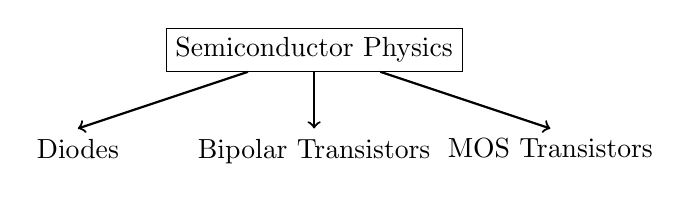
\begin{tikzpicture}
        \node[draw, align=center] (text) {Semiconductor Physics};
        \draw[->, thick] (text) -- ++(0,-1) node[below] {Bipolar Transistors};
        \draw[->, thick] (text) -- ++(-3,-1) node[below] {Diodes};
        \draw[->, thick] (text) -- ++(3,-1) node[below] {MOS Transistors};
    \end{tikzpicture}
\end{center}

We can also redefine Ohm's Law which we know as ($V = IR$) as $J = \sigma \vb{E}$. We can also write resistance($R$) and conductance($G$) in terms of other variables
\begin{gline}
    \item $J$: current density, $A/m^2$ (Amperes per meter squared)
    \item $\sigma$: conductivity, $S/m$ (Siemens per meter)
    \item $\vb{E}$: electric field, $V/m$ (Volts per meter)
\end{gline}

$R = \frac{R}{I} = \rho \frac{l}{A}$ and $G = R^{-1} = \sigma \frac{A}{l}$
\begin{gline}
    \item $\sigma$: conductivity
    \item $\rho$: resistivity
\end{gline}

For collisions in gas, we focus on the idea that initial velocity and direction is lost/randomized after a few collisions. So, when we sum over the random velocities of the particles and average it, it comes out to zero. Average momentum gain is:
\[\bar{\mu} = \frac{\vb{E} q \tau}{M} = \mu \vb{E}, ~~~ \mu := \frac{q \tau}{M} = \frac{\bar{v}}{\vb{E}}\]
\begin{gline}
    \item $\mu$: mobility, $m^2/ (V \cdot s)$
    \item $q$: electric charge, $1.60 \times 10^{-19}$, Coulombs = Amperes/second
    \item $\tau$: mean free time
    \item $M$: mass
    \item $\bar{v}$: average velocity
\end{gline}

Different elements have a different number of outer shell electrons. For semiconductors like silicon, we can increase the temperature to increase its conductivity. Silicon atoms are arranged in a diamond structure and in general, the energy levels that an atom can occupy are discrete. The \textbf{valence band} electrons are at a lower energy state (bound to host atoms) while \textbf{conduction band} electrons are at a higher energy state and are "free" electrons. These electrons are free to move around the crystal and take part in conduction. 

\subsection{Conduction and Fermi Dirac Distribution}
Thermal energy is on average about $\sim 26~eV$ at room temperature How large the \textbf{band-gap}, the gap between the conduction and valence band, determines how conductive a material is:
\begin{itemize}
    \item Insulators: band gap $\sim$ 15 $eV$
    \begin{itemize}
        \item Glass, rubber, oil, plastic, diamond
    \end{itemize}
    \item Semiconductors: band gap $\sim 1 eV$
    \begin{itemize}
        \item Silicon = 1.12 $eV$
    \end{itemize}
    \item Conductors: Not applicable due to overlapping conduction/valence bands
\end{itemize}
This band gap energy is the minumum energy required to break a covalent bond and generate an electron-hole pair.

Because electrons are a type of particle called a \textbf{fermion}, we can say that 
\[f(E) = \frac{1}{e^{\frac{E - E_F}{k_B T}} + 1}\]
\begin{gline}
    \item $f(E)$: occupational probability of a state energy $\epsilon$
    \item $E$: energy of the particle
    \item $E_F$: fermi energy, eV
    \item $k_B$: Boltzmann's constant, $1.380649 \times 10^{-23}$ J/K (Joules per Kelvin), $8.62 \times 10^{-5}$ eV/K
    \item $T$: temperature in Kelvin
\end{gline}

The graph below is a plot of the Fermi-Dirac Distribution at different temperatures. We can use this plot to find the probability of the concentration of electrons ad holes at certain temperatures.
% Source: https://tex.stackexchange.com/questions/251496/fermi-dirac-in-pgfplots-dimension-too-lage

\def\xmax{2.3}\def\ymax{1.2}

\begin{center}
    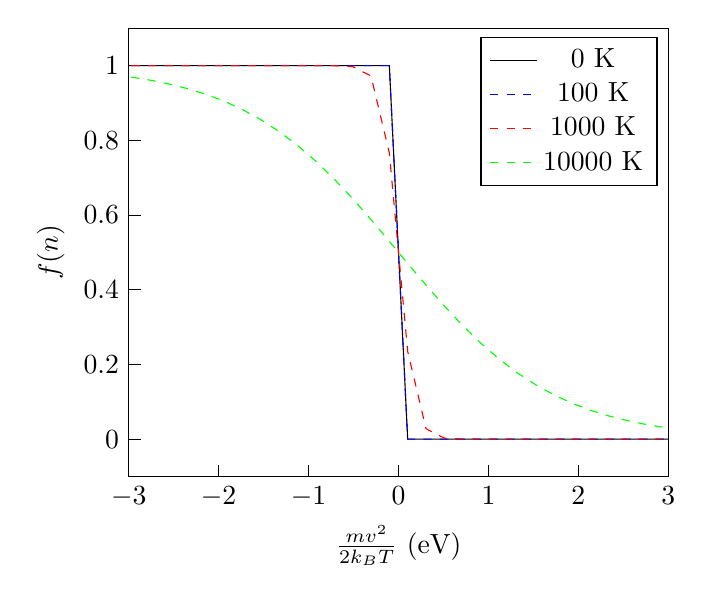
\begin{tikzpicture}
        \begin{axis}[
            xlabel=$\frac{mv^2}{2k_BT}$ (eV),
            ylabel=$f(n)$,
            legend entries={0 K,100 K,1000 K,10000 K},
            x tick style={color=black},
            y tick style={color=black},
            xtick pos=left,
            ytick pos=left,
            xmin=-3,
            xmax=3,
            ymin=-0.1,
            ymax=1.1
            ]
        \addplot[samples=50,black] {(1/((exp((x)/(80.617e-5))+1))};
        \addplot[samples=50,blue,dashed] {(1/((exp((x)/(8.617e-3))+1))};
        \addplot[samples=50,red,dashed] {(1/((exp((x)/(8.617e-2))+1))};
        \addplot[samples=50,green,dashed] {(1/((exp((x)/(8.617e-1))+1))};
        \end{axis}
        \end{tikzpicture}
\end{center}

\textbf{Thermal generation} occurs when sufficient thermal energy exist to break some covalent bonds, which results in a \textbf{free electron}. This free electron is now free to conduct electric current if an electric field is applied to the crystal. However, this leaves behind a net positive charge. \textbf{Holes} are positively charged carrers, which can also move around the crystal and are available to conduct electric current. As temperature increases, so do electron-hole pairs and the conductivity of the crystal. 

\textbf{Recombination} is the process of free electrons and  holes moving through the silicon crystal structure and electrons filling in some of the holes. The recombination rate is proportional to the number of free electrons and holes, which also determines the \textbf{thermal generation} rate.

At thermal equilibrium, $n = p = n_i$. We can alternatively express as
\[pn = n_i^2\]
\begin{gline}
    \item $n$: concentration of free electrons, $cm^{-3}$
    \item $p$: concentration of holes, $cm^{-3}$
    \item $n_i$: number of free electrons nd holes in a unit volume ($cm^3$) of intrinsic silicon at a given temperature
\end{gline}

We can also write $n_i$ as a function of temperature
\[n_i = BT^{3/2} e^{-E_G / 2kT}\]
\begin{gline}
    \item $B$: material-dependent parameter, $7.3 \times 10^{15} \text{cm}^{-3} \text{K}^{-3/2}$ for Silicon
    \item $T$: temperature in $K$
    \item $E_G$: bandgap energy, 1.12 eV for silicon
    \item $k$, Boltzmann's constant
\end{gline}

\subsection{Doping}
In a non-doped crystal like in the above texts, there will be equal concentrations of free electrons and holes from thermal generation. \textbf{Doping} is defined as introducing impurities inside a silicon crystal to adjust the carrier concentration. The following materials are commonly used:
\begin{pline}
    \item Group III elements: boron, aluminum, gallium $\rightarrow$ acceptors; increase holes
    \item Group IV elements: germanium and silicon
    \item Group V elements: phosphorus, arsenic, antimony $\rightarrow$ donors; increase free electrons
\end{pline}
Doping with donors $\rightarrow$ \textbf{n type}.

Doping with acceptors $\rightarrow$ \textbf{p type}

Sometimes we assume that the number of electrons we add is much greater than the original free electrons that pure silicon had ($10^{10}$ per cubic centimeter). This leads to the simplification that the number of free electrons in our silicon crystal is $N_D$, where $N_D$ is the number of donor atoms that we add per cubic centimeter.

\begin{Analysis}{Doping concentrations}{}
Suppose we dope silicon with phosphorus, an acceptor. This means that four electrons from its outer shell will form a covalent bond with silicon. This results in one free electron, meaning that each phosphorus atom donates one free electron to the silicon. No holes are generated during this process. Usually, the concentration of donor atoms, $N_D$, is much greater htan $n_i$, so 
    \[n_n \simeq N_D\]
\begin{gline}
    \item $n_n$: for $n$-type silicon, concentration of free electrons
    \item $p_n$: for $n$-type silicon, concentratation of holes
    \item $N_D$: donor doping concentration
    \item $N_A$: acceptor doping concentration
\end{gline}
$n_n$ is determined by doping concentration, and independent of temperature,  while $p_n$ is determined by:
    \begin{align*}
        p_n n_n &= n_i^2 \\
        p_n &\simeq \frac{n_i^2}{N_D}
    \end{align*}

An analysis with boron, an acceptor, will yield similar conclusions with a change in variables.
\end{Analysis}

\subsection{Practice Problems}
    \begin{enumerate}
        \item Calculate the intrinsic carrier density $n_i$ for silicon at $T = 50$ K and $350$ K.
        \begin{Ans}
            \begin{align*}
                n_{i,1} &= BT^{3/2} e^{-E_G / 2kT} \\
                &= (7.3 \times 10^{15} \text{cm}^{-3} \text{K}^{-3/2})(50 K)^{3/2} e^{-1.12 eV / 2(8.62 \times 10^{-5} eV/K)(50 K)} \\
                &= 9.63217875 \times 10^{-39} / \text{cm}^3 \\
                n_{i,2} &= (7.3 \times 10^{15} \text{cm}^{-3} \text{K}^{-3/2})(350 K)^{3/2} e^{-1.12 eV / 2(8.62 \times 10^{-5} eV/K)(350 K)} \\
                &= 4.15216354 \times 10^{11} / \text{cm}^3
            \end{align*}
        \end{Ans}

        \item Consider an $n$-type silicon for which the dopant concentration $N_D = 10^{17}/\text{cm}^3$. Find the electron and hole concentrations at 350 K. Refer to previous example for the value of $n_i$ at $T = 350$ K.
        \begin{Ans}
            Since this is an $n$-type silicon, 
                \[n_n \simeq N_D = 10^{17} /\text{cm}^3\]
            From this we can find the concentration of minority holes as 
                \[p_n \simeq \frac{n_i^2}{N_D} = \frac{(4.15 \times 10^{11})^2}{10^17} = 1.72 \times 10^6 / \text{cm}^3\]
        \end{Ans}
    \end{enumerate}
\subsection{Sources}
\begin{itemize}
    \item \href{https://www.youtube.com/watch?v=yQDfVJzEymI}{\textcolor{blue}{Razavi Electronics 1, Lec 1, Intro., Charge Carriers, Doping}}
    \item \href{https://file.notion.so/f/f/048d6522-202b-48d4-b5d9-bc005bd602e2/214bf1f0-292f-48d6-9016-737d9f5da155/ee105_reader_v3.pdf?id=237a4300-3dbe-47d1-888b-ffae90d8352b&table=block&spaceId=048d6522-202b-48d4-b5d9-bc005bd602e2&expirationTimestamp=1714435200000&signature=yx-H1qvZJIodPfazOpwXX0Ce2mWMG8skOHl45xoPxus&downloadName=ee105_reader_v3.pdf}{EE105 Reader}
    \item Sedra, Adel S., et al. Microelectronic Circuits. Oxford University Press, 2021
    \item \href{https://eng.libretexts.org/Bookshelves/Materials_Science/TLP_Library_II/22%3A_Introduction_to_Semiconductors/22.2%3A_The_FermiDirac_Distribution}{Engineering LibreTexts: The Fermi-Dirac Distribution}
    \item \href{https://tex.stackexchange.com/questions/251496/fermi-dirac-in-pgfplots-dimension-too-lage}{Fermi-dirac distribution graph}
\end{itemize}

